% 전체 데이터 흐름을 직관적으로 설명하는 Fixed-FK 발표자료
% 컴파일: xelatex calibration_pipeline_overview_fixed_fk.tex (2회)

\documentclass[aspectratio=169,11pt]{beamer}

\usepackage{kotex}
\setmainhangulfont{NanumBarunGothic}
\setsanshangulfont{NanumBarunGothic}
\setmonohangulfont{NanumGothicCoding}
\usepackage{amsmath,amssymb}
\usepackage{booktabs,tabularx,array}
\usepackage{graphicx}
\usepackage{xcolor}

\usetheme{Madrid}
\usecolortheme{whale}
\setbeamertemplate{navigation symbols}{}
\setbeamertemplate{footline}[frame number]
\setbeamerfont{frametitle}{size=\large}
\renewcommand{\arraystretch}{1.25}

\definecolor{fixedblue}{HTML}{2468A2}
\definecolor{gripperorange}{HTML}{D9792B}
\definecolor{fkgreen}{HTML}{3C8D68}
\definecolor{softgray}{HTML}{F2F4F7}

% T_{도착,출발}: 출발 좌표계의 점을 도착 좌표계로 변환
\newcommand{\T}[2]{\mathbf T_{#1,#2}}

\title{멀티카메라 Calibration Pipeline}
\subtitle{PnP·Reprojection·Fixed-FK를 연결한 전체 데이터 흐름}
\author{}
\date{}

\begin{document}

% ------------------------------------------------------------------
\begin{frame}
  \titlepage
\end{frame}

% ------------------------------------------------------------------
\begin{frame}{1. 우리가 구하려는 것}
  \begin{columns}[T]
    \begin{column}{0.48\textwidth}
      \begin{block}{Fixed camera마다 하나}
        \centering
        \Large $\T{B}{C_i}$

        \normalsize
        robot base 기준 camera $i$의 위치와 방향
      \end{block}
    \end{column}
    \begin{column}{0.48\textwidth}
      \begin{block}{Gripper camera에 하나}
        \centering
        \Large $\T{F}{C_g}$

        \normalsize
        flange 기준 gripper camera의 고정된 장착 pose
      \end{block}
    \end{column}
  \end{columns}

  \vfill
  \begin{alertblock}{최종 목표}
    Fixed camera와 gripper camera가 같은 물체를 보았을 때, 모두 robot base 좌표계에서 같은 위치를 말하도록 만든다.
  \end{alertblock}
\end{frame}

% ------------------------------------------------------------------
\begin{frame}{2. 한 번의 촬영에서 저장하는 데이터}
  \begin{columns}[T]
    \begin{column}{0.52\textwidth}
      \begin{itemize}
        \item 각 camera의 RGB image
        \item RGB pixel에 정렬된 aligned depth
        \item 촬영 시각
        \item robot이 제공하는 base-to-flange pose
          \[
            \T{B}{F}^{e}
          \]
        \item set별 raw FK cube pose
          \[
            \T{B}{O}^{s,\mathrm{FK}}
          \]
      \end{itemize}
    \end{column}
    \begin{column}{0.44\textwidth}
      \IfFileExists{cube_in_hand_calibration_setup.png}{%
        \centering
        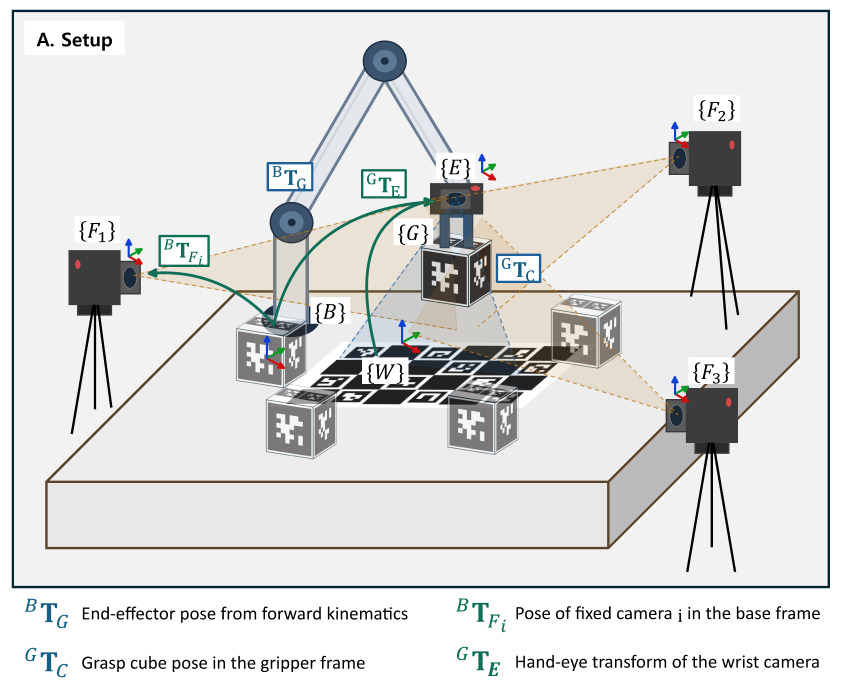
\includegraphics[width=0.88\linewidth,height=0.63\textheight,keepaspectratio]{cube_in_hand_calibration_setup.png}
      }{%
        \begin{block}{데이터 단위}
          Camera $i$\\[2mm]
          Event $e$\\[2mm]
          Set $s$
        \end{block}
      }
    \end{column}
  \end{columns}

  \vfill
  \centering
  저장 전 marker 검출, 임시 PnP, depth 품질과 촬영 시차를 검사하여 불량 event를 제외
\end{frame}

% ------------------------------------------------------------------
\begin{frame}{3. 전체 흐름}
  \begin{columns}[T]
    \begin{column}{0.48\textwidth}
      \begin{enumerate}
        \item \textbf{동기 촬영과 online gate}
        \item \textbf{개별 PnP pose 측정}
        \item \textbf{PnP reprojection 품질 판단}
        \item \textbf{Fixed camera 상대관계 계산}
        \item \textbf{Flange--camera hand--eye}
      \end{enumerate}
    \end{column}
    \begin{column}{0.48\textwidth}
      \begin{enumerate}
        \setcounter{enumi}{5}
        \item \textbf{Robot base에 camera 등록}
        \item \textbf{3D set-pose 일관성 보정}
        \item \textbf{2D raw-corner reprojection 보정}
        \item \textbf{Fixed-FK 전체 동시 최적화}
        \item \textbf{최종 검증과 결과 출력}
      \end{enumerate}
    \end{column}
  \end{columns}

  \vfill
  \begin{alertblock}{흐름의 핵심}
    앞 단계의 출력을 다음 단계의 초기값으로 사용하고, 각 단계에서 오류를 제외·약화·보정한 뒤 더 넓은 범위의
    데이터를 통합한다.
  \end{alertblock}
\end{frame}

% ------------------------------------------------------------------
\begin{frame}{4. 먼저 각 이미지에서 target pose를 측정한다}
  \begin{block}{PnP 입력}
    \centering
    미리 정의한 target의 $N\!\times\!3$ corner
    $+$ RGB에서 검출한 $N\!\times\!2$ pixel
    $+$ camera 내부계수
  \end{block}

  \[
    \T{C_i}{O}^{e}
    =\operatorname{PnP}
    \left(\mathbf X_O,\mathbf u_{i,e},\mathbf K_i,\mathbf D_i\right)
  \]

  \begin{itemize}
    \item 처리 범위: camera 한 대의 event 한 장
    \item 출력: event $e$에서 camera $i$가 본 cube의 3D pose
    \item Cube와 board가 모두 검출되면 각각 별도의 pose를 계산
  \end{itemize}

  \vfill
  \begin{alertblock}{아직 통합 calibration은 아니다}
    이 단계에서는 각 camera가 자기 좌표계에서 target을 어떻게 보았는지만 측정한다.
  \end{alertblock}
\end{frame}

% ------------------------------------------------------------------
\begin{frame}{5. Reprojection error의 역할}
  PnP pose로 3D corner를 다시 영상에 투영한다.

  \[
    \widehat{\mathbf u}_{i,e}^{k}
    =\pi\!\left(\mathbf K_i,\mathbf D_i,
      \T{C_i}{O}^{e}\mathbf X_O^k\right)
  \]
  \[
    \mathbf r_{i,e}^{k}
    =\widehat{\mathbf u}_{i,e}^{k}-\mathbf u_{i,e}^{k}
  \]

  \begin{columns}[T]
    \begin{column}{0.47\textwidth}
      \begin{block}{출력}
        \begin{itemize}
          \item Corner별 pixel residual
          \item 관측 하나의 평균 pixel error
        \end{itemize}
      \end{block}
    \end{column}
    \begin{column}{0.47\textwidth}
      \begin{block}{사용 방법}
        \begin{itemize}
          \item PnP 실패 관측 제외
          \item 여러 pose 후보 중 선택
          \item 불확실한 관측의 영향 감소
        \end{itemize}
      \end{block}
    \end{column}
  \end{columns}

  \vfill
  \centering
  \textbf{이 값은 개별 PnP의 self-fit 품질이며, 최종 multi-camera 정확도는 아니다.}
\end{frame}

% ------------------------------------------------------------------
\begin{frame}{6. 같은 cube로 fixed camera들을 연결한다}
  Camera $i$와 $j$가 같은 event에서 같은 cube를 보았다면:

  \[
    \T{C_i}{C_j}^{e}
    =\T{C_i}{O}^{e}
     \left(\T{C_j}{O}^{e}\right)^{-1}
  \]

  \begin{itemize}
    \item 여러 공통 event에서 camera pair의 상대 pose를 반복 측정
    \item 다른 event들과 크게 어긋나는 측정은 제외
    \item 남은 측정들을 강건하게 통합하여 camera pair당 상대 pose 하나 생성
    \item 여러 camera를 연결했을 때 관계가 서로 모순되지 않는지 확인
  \end{itemize}

  \vfill
  \begin{block}{이 단계의 결과}
    Fixed camera들이 \textbf{서로 어떻게 배치됐는지}는 알지만, 아직 robot base에서 어디에 있는지는 모른다.
  \end{block}
\end{frame}

% ------------------------------------------------------------------
\begin{frame}{7. 여러 event로 hand--eye를 구한다}
  \begin{columns}[T]
    \begin{column}{0.48\textwidth}
      \begin{block}{Robot이 제공}
        Event별 flange pose
        \[
          \T{B}{F}^{e}
        \]
      \end{block}
    \end{column}
    \begin{column}{0.48\textwidth}
      \begin{block}{Gripper camera가 관측}
        Event별 target PnP pose
        \[
          \T{C_g}{O}^{e}
        \]
      \end{block}
    \end{column}
  \end{columns}

  \vfill
  서로 다른 event의 상대운동이 일치하도록 hand--eye 식을 푼다.
  \[
    \mathbf A_{ab}\mathbf X=\mathbf X\mathbf B_{ab},
    \qquad \mathbf X=\T{F}{C_g}
  \]

  \begin{alertblock}{출력}
    $\T{F}{C_g}$ 하나: gripper camera가 flange에 어디에, 어떤 방향으로 장착됐는가
  \end{alertblock}

  \small
  다른 event들과 크게 어긋나는 pose는 제외하고, 여러 hand--eye 해 중 전체 motion에서 가장 일관적인 결과를
  선택한다. Robust refinement가 오차를 개선하지 못하면 초기 hand--eye 결과를 유지한다.
\end{frame}

% ------------------------------------------------------------------
\begin{frame}{8. Fixed camera를 robot base에 등록한다}
  Gripper camera의 event별 base pose:
  \[
    \T{B}{C_g}^{e}=\T{B}{F}^{e}\T{F}{C_g}
  \]

  Gripper camera가 본 cube의 base pose:
  \[
    \T{B}{O}^{g,e}
    =\T{B}{F}^{e}\T{F}{C_g}\T{C_g}{O}^{e}
  \]

  Fixed camera가 본 cube의 base pose:
  \[
    \T{B}{O}^{i,e}
    =\T{B}{C_i}\T{C_i}{O}^{e}
  \]

  \vfill
  이 공통 target을 통해 fixed-camera pose $\T{B}{C_i}$의 초기값을 계산한다. Board 경로와 cube 경로가 모두
  있으면 event 간 변동이 더 작은 경로를 선택하고, 두 결과가 충분히 가까울 때만 결합한다. 크게 다른 경로를
  무리하게 평균내지 않는다.
\end{frame}

% ------------------------------------------------------------------
\begin{frame}{9. 3D pose 수준의 set 일관성 보정}
  같은 set에서 고정된 cube는 어느 fixed camera로 계산하더라도 같은 base pose가 나와야 한다.

  \[
    \T{B}{O}^{i,e}=\T{B}{C_i}\T{C_i}{O}^{e}
  \]

  Fixed-FK에서는 이 값을 raw FK cube pose와 비교한다.
  \[
    \T{B}{O}^{i,e}\approx\T{B}{O}^{s,\mathrm{FK}}
  \]

  \begin{itemize}
    \item 반복적으로 같은 방향으로 어긋나는 camera: $\T{B}{C_i}$ 보정량 계산
    \item 수정량이 작고 일관성이 좋아짐: 전부 적용
    \item 수정량이 다소 큼: 일부만 적용
    \item 수정량이 비정상적으로 큼: 보정 결과를 거부하고 이전 값 유지
  \end{itemize}

  \begin{block}{사용하는 오차}
    2D pixel이 아니라 PnP로 얻은 3D pose의 위치·방향 불일치
  \end{block}
\end{frame}

% ------------------------------------------------------------------
\begin{frame}{10. 2D raw-corner reprojection 보정}
  D2의 camera pose를 초기값으로 사용하고, event별 object pose는 고정한다.

  \[
    \widehat{\mathbf u}_{i,e}^{k}
    =\pi\!\left(
      \mathbf K_i,\mathbf D_i,
      \left(\T{B}{C_i}\right)^{-1}\T{B}{O}^{e}\mathbf X_O^k
    \right)
  \]

  \[
    \min_{\T{B}{C_i}}
    \sum_{e,k}\rho\!\left(
      \left\|\widehat{\mathbf u}_{i,e}^{k}-\mathbf u_{i,e}^{k}\right\|^2
    \right)
  \]

  \begin{itemize}
    \item 최적화 변수: fixed-camera pose $\T{B}{C_i}$
    \item 비교값: 예측 corner와 실제 RGB 검출 corner
    \item 큰 corner 오차: robust loss로 영향 감소
    \item Pixel RMSE가 좋아지지 않거나 pose 변화가 과도함: 결과 거부
  \end{itemize}

  \begin{alertblock}{D2와 D3의 차이}
    D2는 3D pose 일관성, D3는 원본 2D pixel 일치도를 이용해 같은 camera pose를 단계적으로 정밀화한다.
  \end{alertblock}
\end{frame}

% ------------------------------------------------------------------
\begin{frame}{11. Fixed-FK: cube pose를 고정 기준으로 사용}
  Robot은 set $s$의 cube pose를 FK로 제공한다.
  \[
    \boxed{\T{B}{O}^{s,\mathrm{FK}}}
  \]

  \begin{alertblock}{Fixed-FK의 가정}
    Raw FK cube pose가 정확하다고 보고, vision으로 수정하지 않으며 최적화 중에도 움직이지 않는다.
  \end{alertblock}

  따라서 두 camera 경로가 모두 동일한 FK cube pose를 설명해야 한다.
  \[
    \T{B}{C_i}\T{C_i}{O}^{e}
    \approx \T{B}{O}^{s,\mathrm{FK}}
  \]
  \[
    \T{B}{F}^{e}\T{F}{C_g}\T{C_g}{O}^{e}
    \approx \T{B}{O}^{s,\mathrm{FK}}
  \]
\end{frame}

% ------------------------------------------------------------------
\begin{frame}{12. 전체 시스템 동시 최적화}
  \begin{columns}[T]
    \begin{column}{0.47\textwidth}
      \begin{block}{고정하는 값}
        \begin{itemize}
          \item Raw FK cube pose $\T{B}{O}^{s,\mathrm{FK}}$
          \item Event별 flange pose $\T{B}{F}^{e}$
          \item 선택된 PnP 관측
        \end{itemize}
      \end{block}
    \end{column}
    \begin{column}{0.47\textwidth}
      \begin{block}{동시에 최적화하는 값}
        \begin{itemize}
          \item 모든 fixed-camera pose $\T{B}{C_i}$
          \item Hand--eye $\T{F}{C_g}$
          \item 고정 board pose $\T{B}{W}$
        \end{itemize}
      \end{block}
    \end{column}
  \end{columns}

  \vfill
  \begin{center}
    Fixed camera residual
    $+$ gripper camera residual
    $+$ board residual
    $+$ camera 간 residual

    \Large $\Downarrow$

    \normalsize 전체 residual이 최소가 되도록 calibration 행렬을 함께 수정
  \end{center}

  \vfill
  \small 여기서 ``동시(joint)''는 robot joint가 아니라 여러 calibration 변수를 함께 푼다는 뜻이다.
\end{frame}

% ------------------------------------------------------------------
\begin{frame}{13. 오차는 단계에 따라 다르게 처리한다}
  \begin{tabularx}{\textwidth}{>{\bfseries}p{0.19\textwidth}X X}
    \toprule
    처리 & 언제 사용하는가 & 의미 \\
    \midrule
    제외 & 검출 실패, PnP 실패, 명확한 outlier & 이후 계산에 사용하지 않음 \\
    선택 & 가능한 PnP pose가 여러 개 & 가장 일관적인 pose를 사용 \\
    영향 감소 & 사용 가능하지만 불확실한 관측 & Robust loss 또는 작은 가중치로 반영 \\
    최적화 & 여러 camera 관계가 조금씩 불일치 & Calibration transform을 수정 \\
    결과 거부 & 최적화 후 오차가 개선되지 않거나 pose 변화가 과도함 & 최적화 전 단계 결과를 유지 \\
    검증 & 최종 calibration 평가 & 결과를 수정하지 않고 오차를 보고 \\
    \bottomrule
  \end{tabularx}
\end{frame}

% ------------------------------------------------------------------
\begin{frame}{14. 최종 검증과 핵심 정리}
  \begin{columns}[T]
    \begin{column}{0.48\textwidth}
      \begin{block}{최종 검증}
        \begin{itemize}
          \item Cross-camera cube pose 일관성
          \item Hand--eye와 robot motion 일관성
          \item Marker reprojection error
          \item Depth 표면과 cube 크기 검증
        \end{itemize}
      \end{block}
    \end{column}
    \begin{column}{0.48\textwidth}
      \begin{block}{Depth의 역할}
        \begin{itemize}
          \item 촬영 품질 검사
          \item PnP pose의 표면 일관성 확인
          \item 최종 물리 크기 검증
          \item 기본 PnP reprojection 식에는 직접 사용하지 않음
        \end{itemize}
      \end{block}
    \end{column}
  \end{columns}

  \vfill
  \begin{alertblock}{한 문장 요약}
    각 이미지에서 PnP pose를 측정한 뒤, raw FK cube pose를 공통의 고정 기준으로 두고 fixed camera와 gripper
    camera의 calibration 행렬을 전체 관측에 동시에 맞춘다.
  \end{alertblock}
\end{frame}

\end{document}
